% Chapter 1

\chapter{Introduction} % Write in your own chapter title
\label{Chapter1}

Delay tolerant network(DTN) architecture lacks continuous end to end
connectivity. It works under some constraints like long delays and
extreme losses. For example, military network having large number of
nodes with high data mobility in extreme environmental terrestrial
conditions. Such network normally employees their own tailored routing
algorithm for high throughput based on individual's environmental
conditions~\cite{1}.\\
Now if we need to transfer image over such wireless delay tolerant
network, and that too from a live camera then it is going to become
extremely difficult task.Complexity will increases further, if we need
to build a viable low cost system with a low power battery operated
solution.  In any such cases, it would be wise to transmit
information only.We need to extract information out of image and then to
send it over the network.  Information can be of various type. So, we
need to deal that what minimum information about image allows us to
reconstruct the scenario or to detect an event. If possible then we 
need to detect event at the end DTN node itself and then to transmit
only this event information over the network.\\
Above discussed image pipeline system can also be extended to
the existing video surveillance system which are still manual. Normally
all the surveillance camera sends video to a monitoring base station,
where it is monitored by a person or a group of person. But such
arrangement can not be foolproof. So, any attempt in the direction of
its automation can be of great use in application areas such as:
\begin{enumerate}
 \item  Traffic Monitoring
  \item Elderly care
  \item Security
  \item Surveillance
  \item Assembly Line Inspection
\end{enumerate}
End goal of such an intelligent system would be to offer an
automatic analysis of scene and then to infer desired information out of
it.These systems can be lot complex because of the complexity of the
scene, specially when application is targeted for outdoor monitoring.
Sometime background of the scene can be moving, while in some
other scene ambient light can be different. Detection of foreground
objects becomes a trivial task in whole of this pipeline.Once we have
foreground objects, we can save a lot of bandwidth if we can detect if
object is of our interest or not.\\
In the current work, we are targeting to detect moving person and
then to send it's information such as location, time of detection etc to
the monitoring station. We want to keep our pipeline computation cost
very low, at the same time with high genuine detection rate and low
false detection rate.


\section{Past Work and Literature Survey}

\subsection{Image transfer over DTN/Low BW networks}

There has been no data available for the image transfer over terrestrial
DTNs, however there has been several attempts ~\cite{2, 3, 4, 5} to transfer
image over low bandwidth wireless sensor networks (WSN).

Georgiy et al. ~\cite{2} have tried to transfer different versions of JEPG
images over zigbee network and then has done performance comparison.
This works shows that there is an effect of compression coding algorithm
on peak signal to noise ratio(PSNR). It has been observed that
compression technique with scalable coding is more error tolerant in WSN
environment.Hengstler et al. ~\cite{3, 5} have gone step ahead and have used 3
cameras. One high resolution camera and two low resolution cameras. Low
resolution cameras are used for stereo matching and to identify any
moving object in the camera's field of view (FOV). If a moving object is
found then only high resolution camera is triggered. Such system is
power efficient in  comparison to the camera mote continuously
transmitting JPEG frames. Chen et al. ~\cite{4} have used xetal parallel
processors for image processing. After subtracting background, ellipse
fitting has been done on the foreground object. This elliptical
information is collected from different camera and 3D view is
reconstructed from it. 

\begin{figure}[!b]
\centering
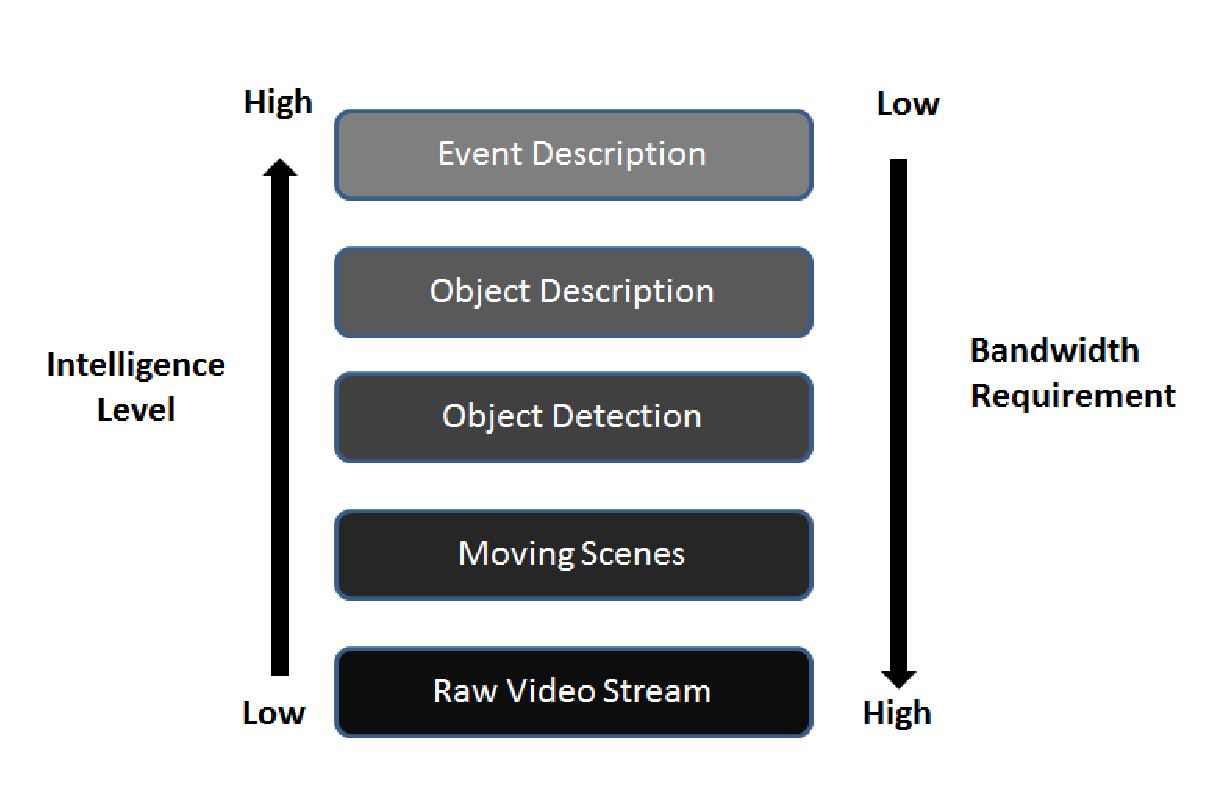
\includegraphics[scale=0.80]{Figures/image_tr_level}
\caption{Surveillance image transfer level, reproduced from ~\cite{3}}
\label{image_tr_level}
\end{figure}

Figure ~\ref{image_tr_level} shows different level of intelligence at
which data can be transmitted in an augmented video surveillance
system. As we go above in the hierarchy, we attain higher level of
intelligence and save lot of bandwidth. But all these come at the cost
of computational power of mote node.

\subsection{Image size reduction techniques}
Most of the image intensity information are not distinguishable by human
eye, so they are irrelevant. Normally, neighbouring pixel of an image
are co-related to each other, so they are redundant. Such redundancy is
called spatial redundancy.Coming to the video, they are composed of
large number of still images , which have been taken at very short
interval of time. So, it is expected that there would be lot of temporal
redundancy between two neighbouring frames.  Therefore an image
compression technique is developed around basic principal of reducing
irrelevancy and redundancy. Broadly, compression techniques are
categorised in lossless and lossy ~\cite{6}. In a lossless compression, original
image can be retrieved exactly, but it does not gives much compression.
Reconstructed image after a lossy compression degrades in quality,
however they provide good amount of compression. We do not need to
reconstruct exact image for surveillance applications. So maximum
possible compression would help a lot of bandwidth on network.\\

Most of the video coding method are based on transform coding followed
by predictive coding based on motion estimation. Such methods are called
block based method, where prediction is implemented on a complete block.
MPEG-1,2 come in this category. However,algorithm based on object based
coding techniques ~\cite{7, 8} including MPEG-4 provides substantially
better compression. Chaudhury et al. ~\cite{7} have used principal
component analysis (PCA) method for object segmentation.Further, they
have reused tracking subspace for object coding which substantially
reduced computational time. Babu et al. ~\cite{8} have calculated motion
between current and previous frame. Further motion compensated error and
other object parameters such as boundary, location and motion
information has been coded using suitable source coding techniques.  

\subsection{Background subtraction techniques}
In any object based method, focus is on foreground object (FG) which is part
of actual information.The most simple way of getting FG objects is to
find difference with the previous frame. Offcourse it is computationally
least expensive , but does not work for most of the practical
cases. Basic of all background (BG) modeling algorithm is to find an
image pattern which does not have any moving object. However, this is a
very complex task, as sometimes camera itself might be moving, in some
other cases lighting condition can vary a lot.In some cases even all the
moving objects might not be of interest. For example, escalator is the
part of BG in a scene where a person is standing on a moving
escalator.\\
Many methods ~\cite{9, 10, 11, 12, 13, 14} have been developed for the background
subtraction (BGS), having strength and weakness in terms of computation
complexities and performance. Frame differencing is of lowest
computational complexity. Here simply current frame is subtracted with
the last frame, and if absolute of the subtracted value is less than a
threshold value, then that pixel is made part of BG. Biggest drawback of
this method is that if an FG object stays for more than a frame time at
any position then that is made part of BG. Further, if an FG object is
consist of almost uniformly distributed intensities, then internal
portion of the object is considers as BG. However, there is one biggest
advantage of this method is that, it is quickly adaptable to the change
in scene, as it depends on only last frame.\\
BGS algorithm ~\cite{10, 12, 13, 14} based on Gaussian average or median of
last couple of frames, comes in the category of middle level of
computational cost. Wren et al. ~\cite{12} have used running average of
last n frames as BG model. Algorithms based on median filter show better
performance, but it has more memory requirement compared to running
average. Here, median of last n pixel is considers as BG model.
McFarlane et al. ~\cite{14} have used modified version as average median
filter, which has memory requirement same as that of frame differencing.
Here, if a pixel value is greater than the corresponding BG pixel, then
BG pixel value is incremented by 1, and if it is less then decremented
by 1.\\
Yao et al. ~\cite{11} have used a method based on local texture features
represented by local binary patterns (LBP) and photometric invariant
color measurements in RGB color space. Texture is an important
characteristic of images and video. LBP is invariant to any monotonic
gray level change. Also, it is computationally very simple. LBP operator
labels image pixel of a cell by thresholding the neighborhood of each pixel
with the center value and considering the result as a binary number.

LBP binary code of a pixel is calculated as follows:
\begin{equation}
LBP_{NR} = \Sigma _{n = 0} ^{N - 1} f(I_c - I_n) 2^n \hspace{20 mm} where f(x) = \left\{ 
  \begin{array}{l l}
     1 & \quad \text{if $x$ $\geq$  $0$}\\
     0 & \quad \text{otherwise}
   \end{array} \right.
\end{equation}
Here, $I_c$ is the gray value of central pixel and I$_n$ are the gray
value of pixels at a distance of radius R.  On a multi channel color
image LBP can be calculated at each pixel separately.LBP works well with
local illumination changes, however there can be issues in case of
global illumination change.LBP fails when both background and foreground
of an image shares same texture information. Yao et al. have used
photometric invariant color features in RGB color space to overcome this
limitation of LBP.

\subsection{Object detection techniques}

\subsection{Outstanding issues}

\section{Motivation}
what and why I will do?

\section{Organisation of thesis}
